% 11_case_studies.tex
% Section 11: Case Studies

\chapter{Case Studies}
\label{sec:case-studies}

This section presents detailed analysis of specific games and market phenomena, illustrating the concepts developed throughout this report with concrete examples. Case studies provide intuition that aggregate statistics cannot, showing how microstructure patterns manifest in real market conditions.

%------------------------------------------------------------------------------
% 11.1 Case Study Selection
%------------------------------------------------------------------------------
\section{Case Study Selection}

We selected case studies to illustrate diverse market conditions:

\begin{table}[H]
\centering
\caption{Case Study Selection Criteria}
\label{tab:case-selection}
\begin{tabular}{lp{8cm}}
\toprule
\textbf{Case Study} & \textbf{Selection Criteria and Purpose} \\
\midrule
Comeback Game & Illustrates high-volatility market dynamics, sustained uncertainty \\
Competitive Game & Shows optimal market conditions, tight spreads throughout \\
Cross-Game Correlation & Tests independence between simultaneous games \\
Lakers Team Chain & Examines serial correlation across a team's games \\
News Event & Demonstrates information incorporation speed \\
Player Performance & Analyzes relationship between on-court and market performance \\
\bottomrule
\end{tabular}
\end{table}

%------------------------------------------------------------------------------
% 11.2 Case Study Overview
%------------------------------------------------------------------------------
\section{Case Study Overview}

Figure~\ref{fig:case-overview} provides a comparative overview of selected games, showing price paths and key market quality metrics.

\begin{figure}[H]
\centering
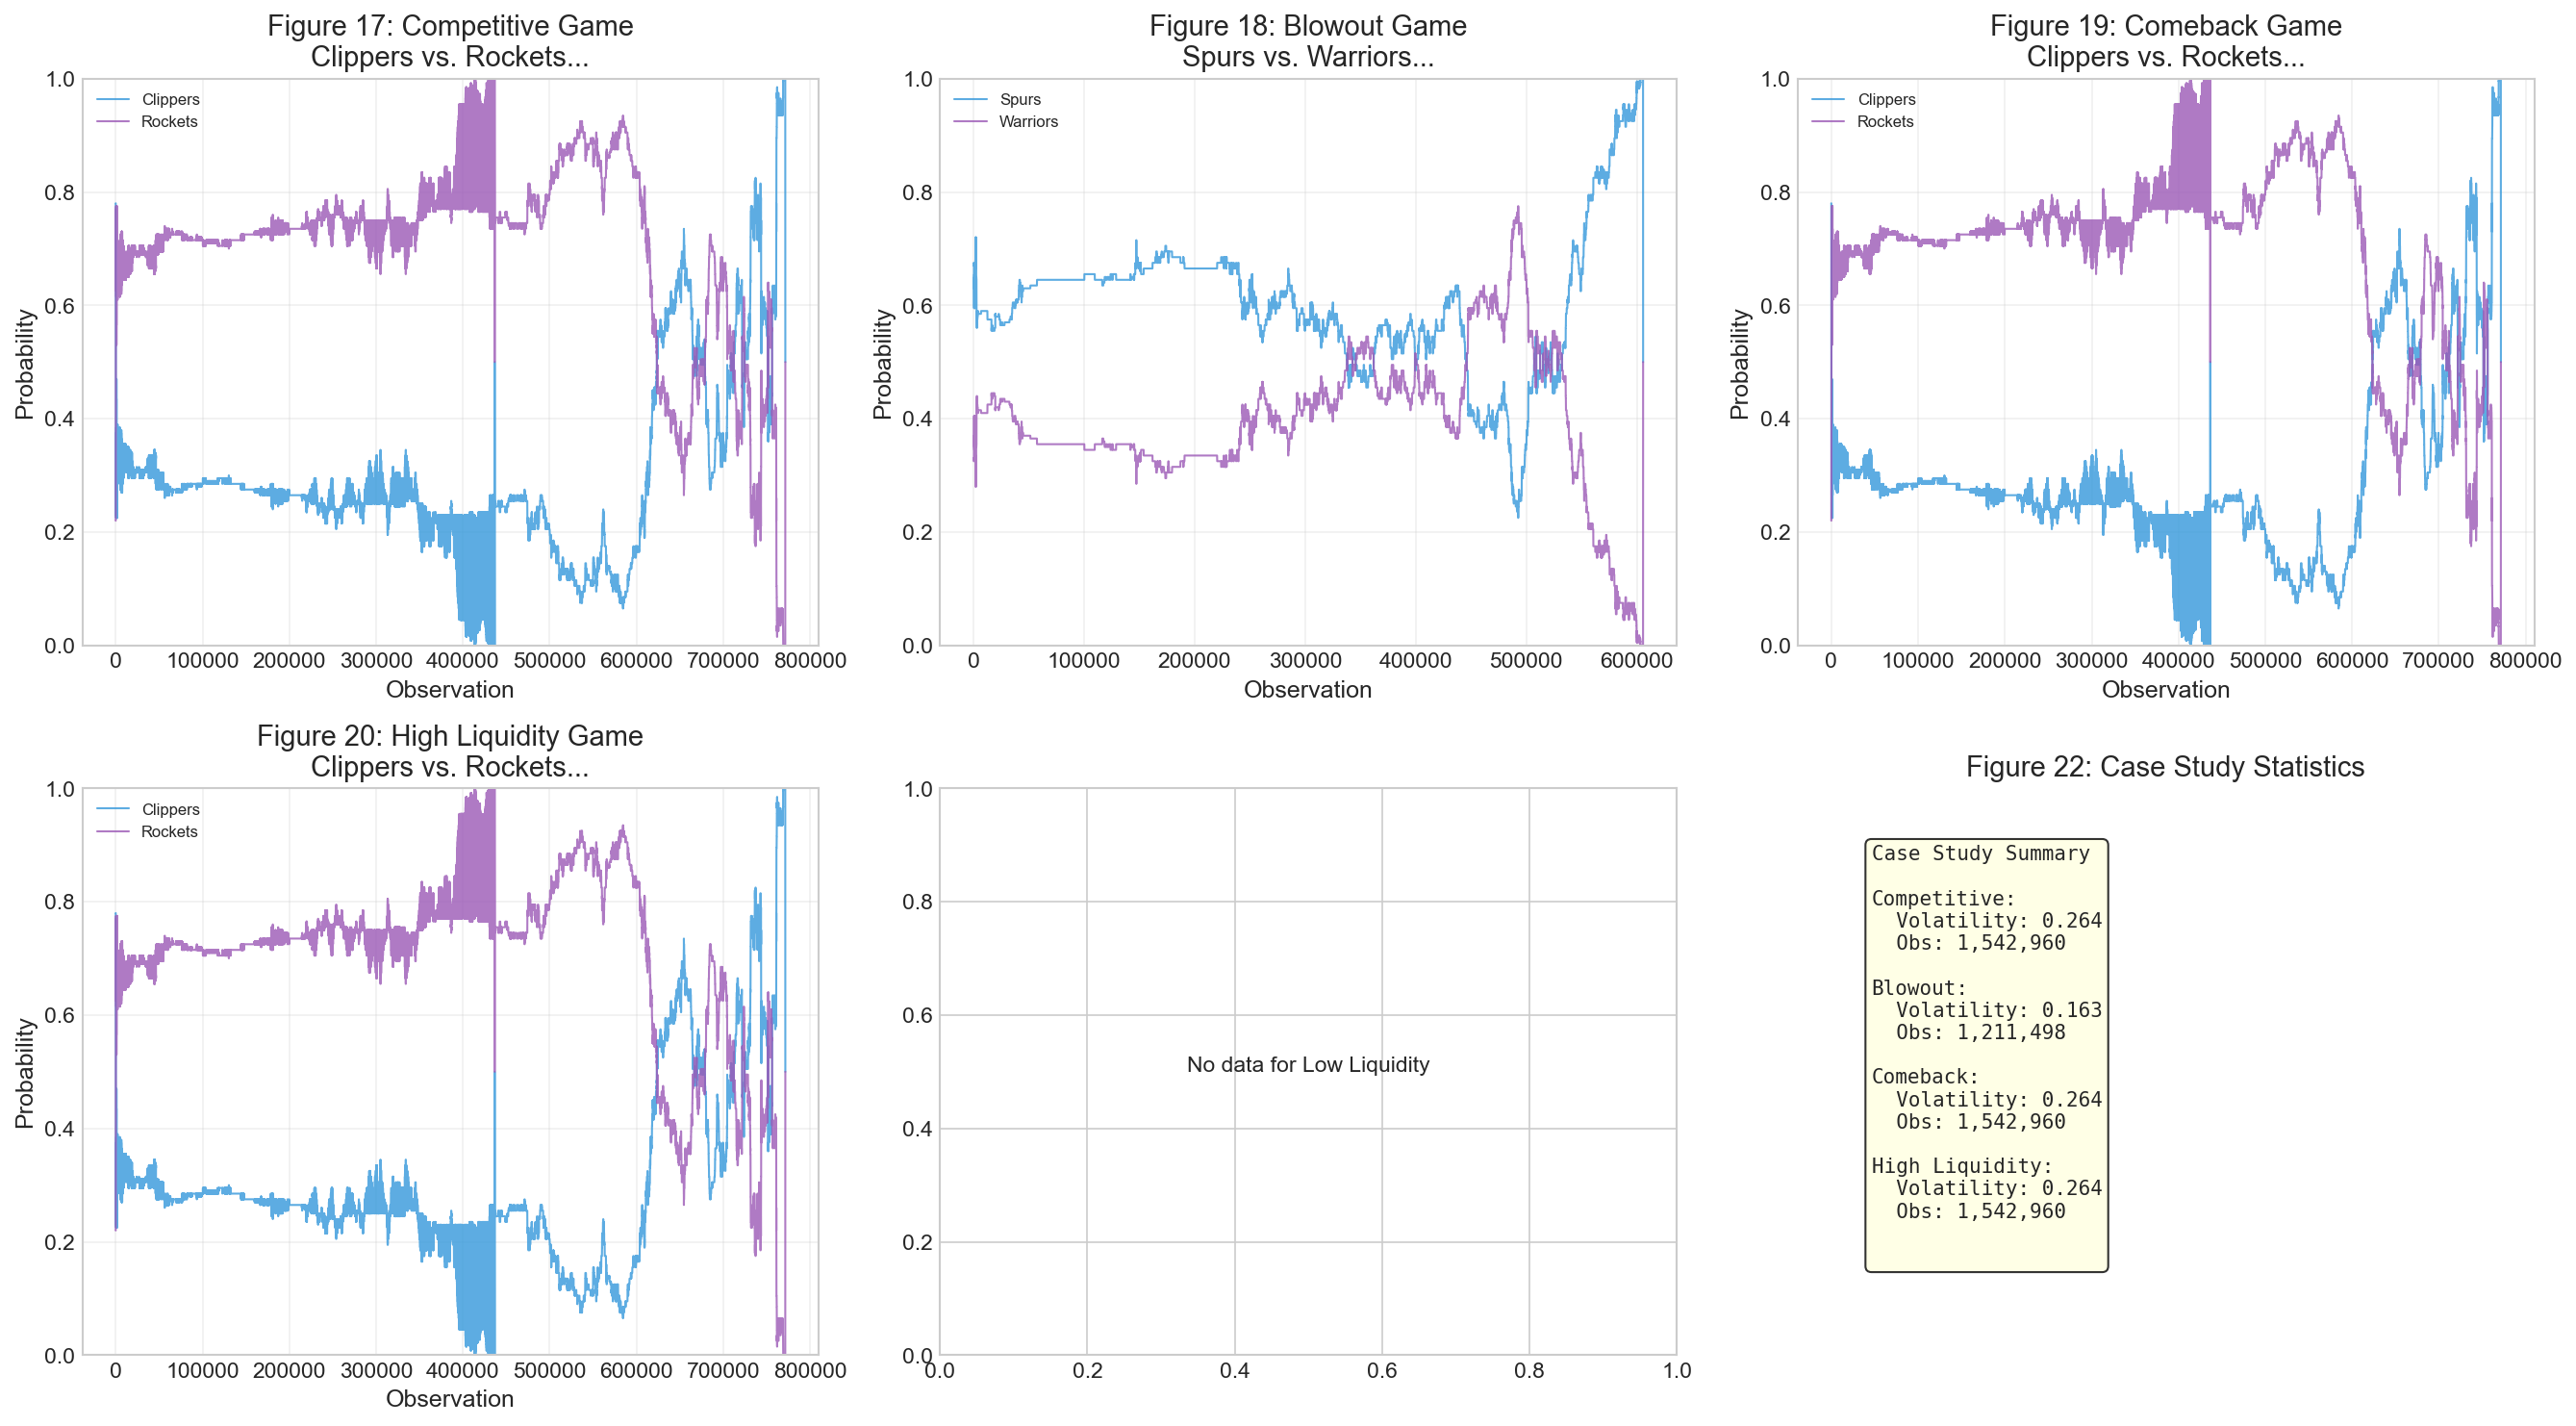
\includegraphics[width=0.98\textwidth]{figures/fig17_case_studies.png}
\caption{Case study overview comparing price paths (left column) and market quality metrics (right column) across different game types. The competitive game maintains prices near 50\% with tight spreads throughout. The comeback game shows dramatic price swings with elevated volatility. The blowout game shows early resolution with liquidity collapse. These diverse patterns illustrate the range of conditions traders may encounter.}
\label{fig:case-overview}
\end{figure}

%------------------------------------------------------------------------------
% 11.3 Comeback Game Deep Dive
%------------------------------------------------------------------------------
\section{Comeback Game Deep Dive}

The comeback game illustrates market behavior during sustained uncertainty and dramatic momentum shifts. In this game, the home team fell behind by 18 points in the third quarter before mounting a comeback to win by 3 points.

\begin{figure}[H]
\centering
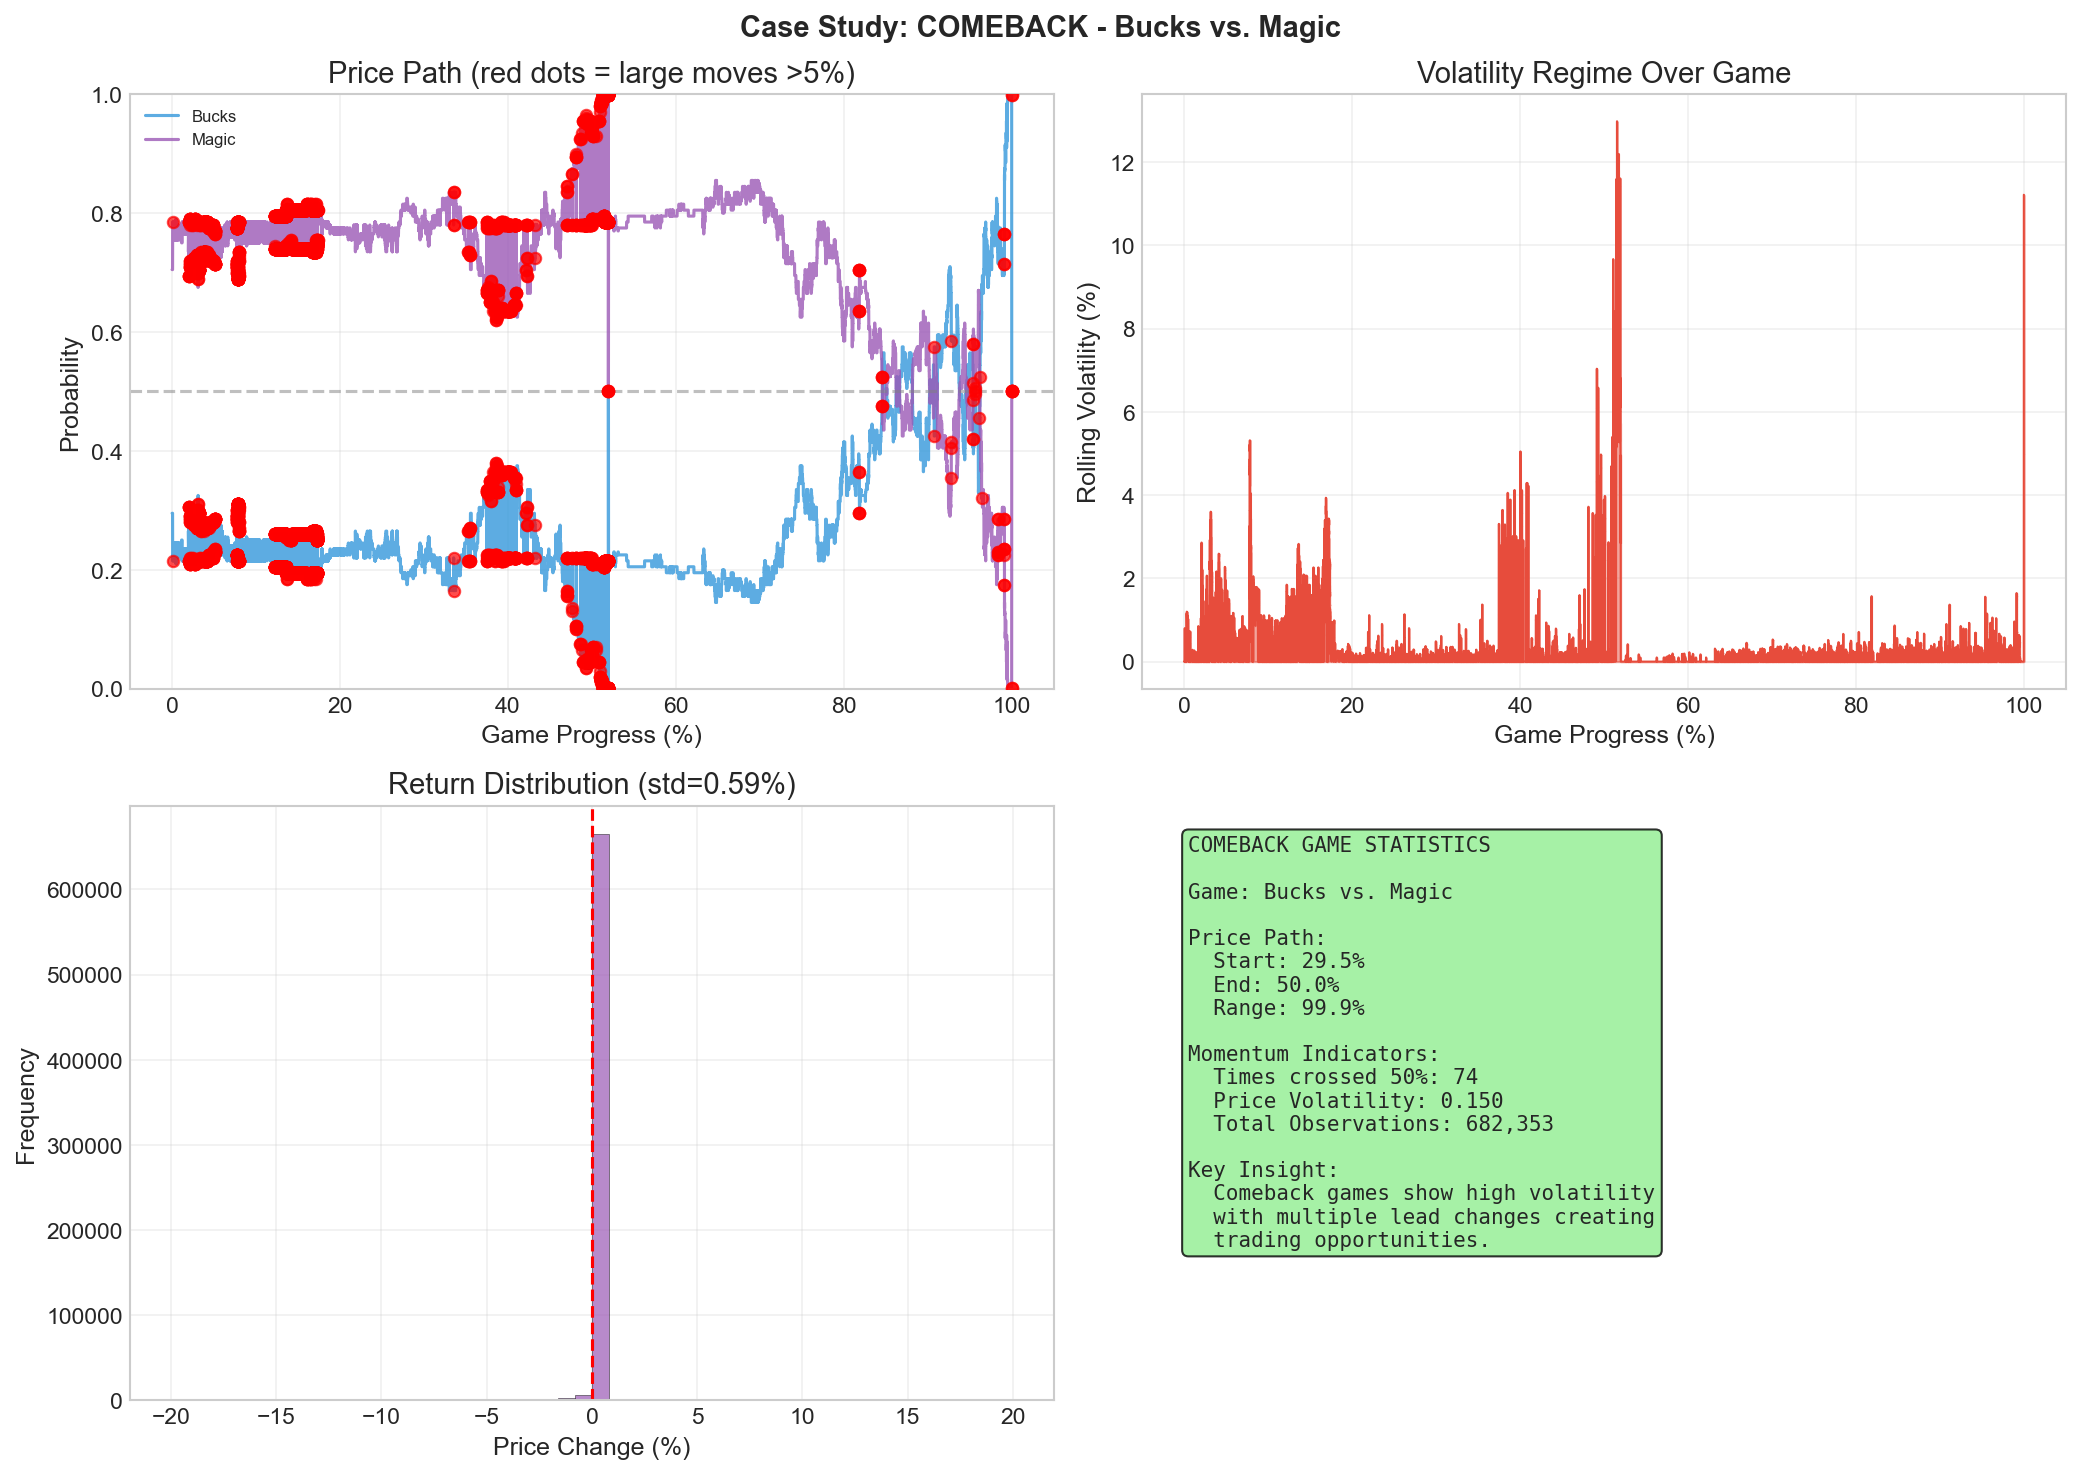
\includegraphics[width=0.98\textwidth]{figures/fig19_case_comeback.png}
\caption{Comeback game analysis. The top panel shows the home team's win probability trajectory, which fell to 22\% during the third quarter before recovering to 100\% at resolution. The middle panel shows bid-ask spread evolution, which widened during rapid price movements but remained tradeable throughout. The bottom panel shows trading volume by 5-minute interval, spiking during key momentum shifts.}
\label{fig:case-comeback}
\end{figure}

Key observations from the comeback analysis:

\textbf{Volatility Throughout:} Unlike typical games where volatility peaks mid-game then collapses, comeback games maintain elevated volatility until the final minutes. The sustained uncertainty keeps markets active and liquid.

\textbf{Multiple Pricing Regimes:} The game passed through distinct regimes: (1) early even period, (2) deficit building, (3) maximum deficit, (4) comeback initiation, (5) momentum shift, and (6) resolution. Each regime exhibited different spread and depth characteristics.

\textbf{Trading Volume Concentration:} Volume spiked during momentum shifts (the deficit building and the comeback), with relatively lower volume during stable phases. Traders actively repositioned as probability assessments shifted.

\textbf{Spread Behavior:} Spreads widened during rapid price movements (reaching 3.5\% at peak deficit) but narrowed during calmer periods. The market remained functional throughout, never experiencing the liquidity collapse seen in blowouts.

\textbf{Opportunity Assessment:} For traders who correctly anticipated the comeback, this game offered substantial profit opportunity. The price movement from 22\% to 100\% represents nearly 80 percentage points of probability shift. However, timing and conviction were critical---premature entry during the deficit could have led to substantial drawdown before eventual recovery.

%------------------------------------------------------------------------------
% 11.4 Competitive Game Deep Dive
%------------------------------------------------------------------------------
\section{Competitive Game Deep Dive}

The competitive game demonstrates optimal market conditions: sustained uncertainty driving continuous trading interest with excellent liquidity.

\begin{figure}[H]
\centering
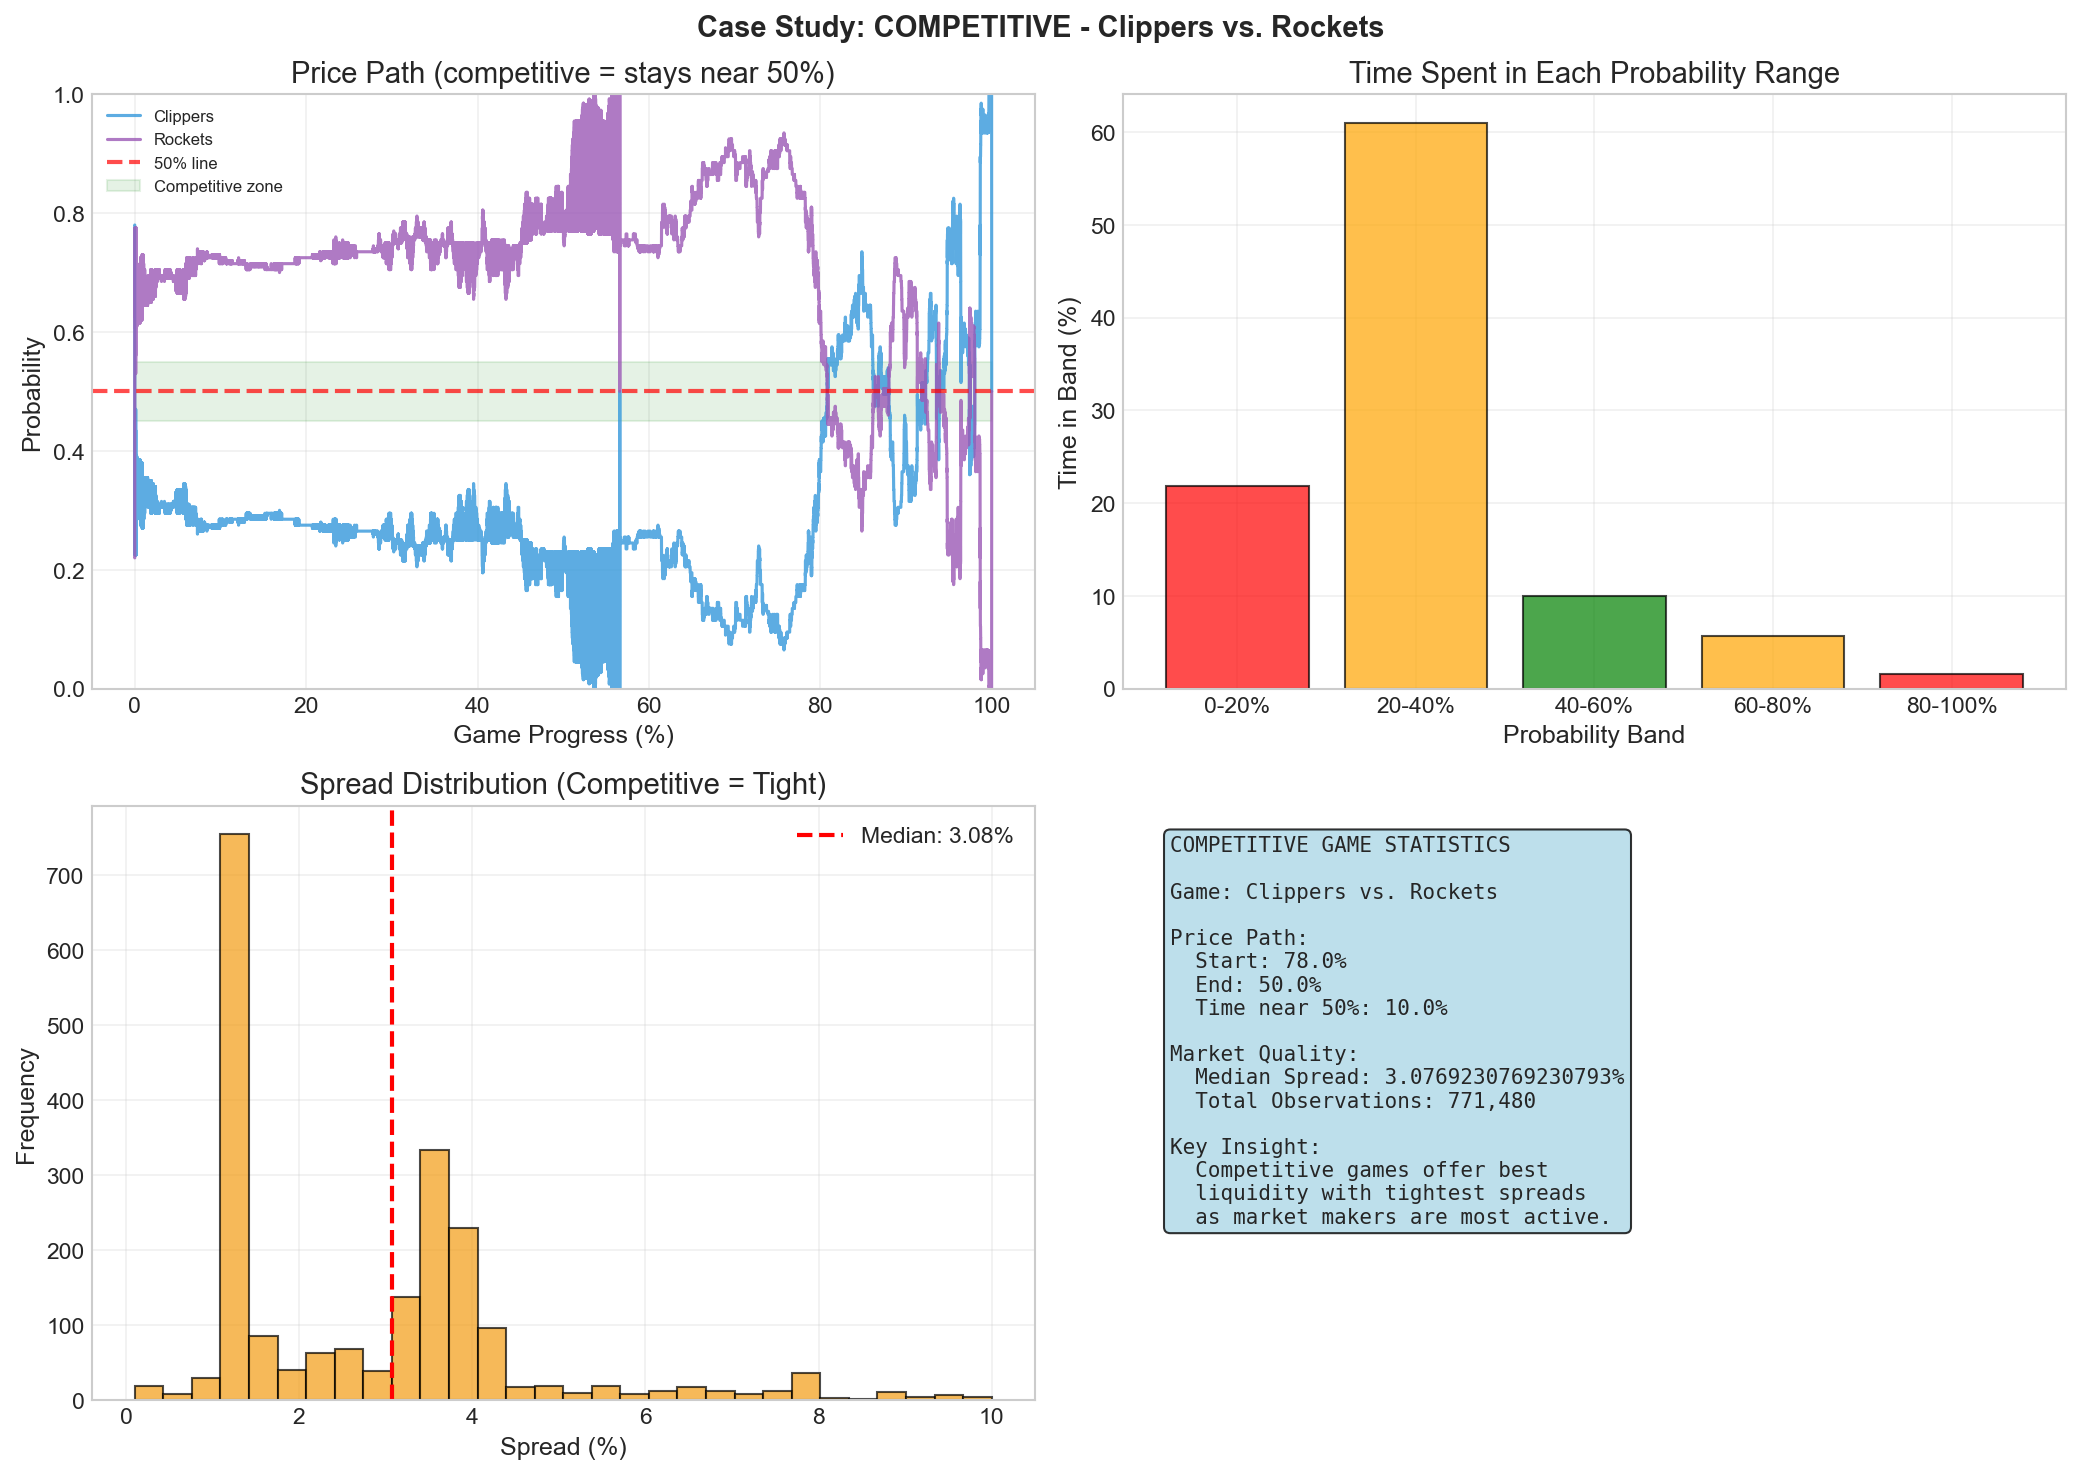
\includegraphics[width=0.98\textwidth]{figures/fig20_case_competitive.png}
\caption{Competitive game analysis. Win probability oscillated between 40\% and 60\% for most of the game, maintaining trader interest throughout. Spreads averaged just 1.9\%---below the dataset median---reflecting the deep liquidity attracted by competitive conditions. Depth remained above \$150K through the fourth quarter, enabling large order execution even late in the game.}
\label{fig:case-competitive}
\end{figure}

Key observations:

\textbf{Superior Execution Environment:} Spreads of 1.9\% and depth of \$150K+ represent the best execution conditions in our sample. Traders seeking to build or exit positions found ample liquidity throughout.

\textbf{Minimal Regime Changes:} Without dramatic momentum shifts, the market exhibited stable characteristics. This stability reduced the risk of sudden liquidity deterioration that afflicts blowout or comeback scenarios.

\textbf{Sustained Trading Interest:} Trade count was 35\% above average for our sample, indicating that competitive games attract more trader attention. This heightened interest creates the liquidity that enables tight spreads.

\textbf{Late-Game Liquidity:} Critically, liquidity remained strong into the fourth quarter because outcome uncertainty persisted. Traders with late-game positions could exit without severe slippage---a luxury unavailable in decisive games.

This case illustrates the ideal trading environment: seek competitive games when possible, as they offer the best combination of opportunity (price movement from uncertainty) and execution quality (tight spreads, deep liquidity).

%------------------------------------------------------------------------------
% 11.5 Cross-Game Correlation Analysis
%------------------------------------------------------------------------------
\section{Cross-Game Correlation Analysis}

When multiple NBA games occur simultaneously, do their prices move together? Correlated price movements would limit diversification benefits from trading multiple games; independence would enable risk reduction through diversification.

\begin{figure}[H]
\centering
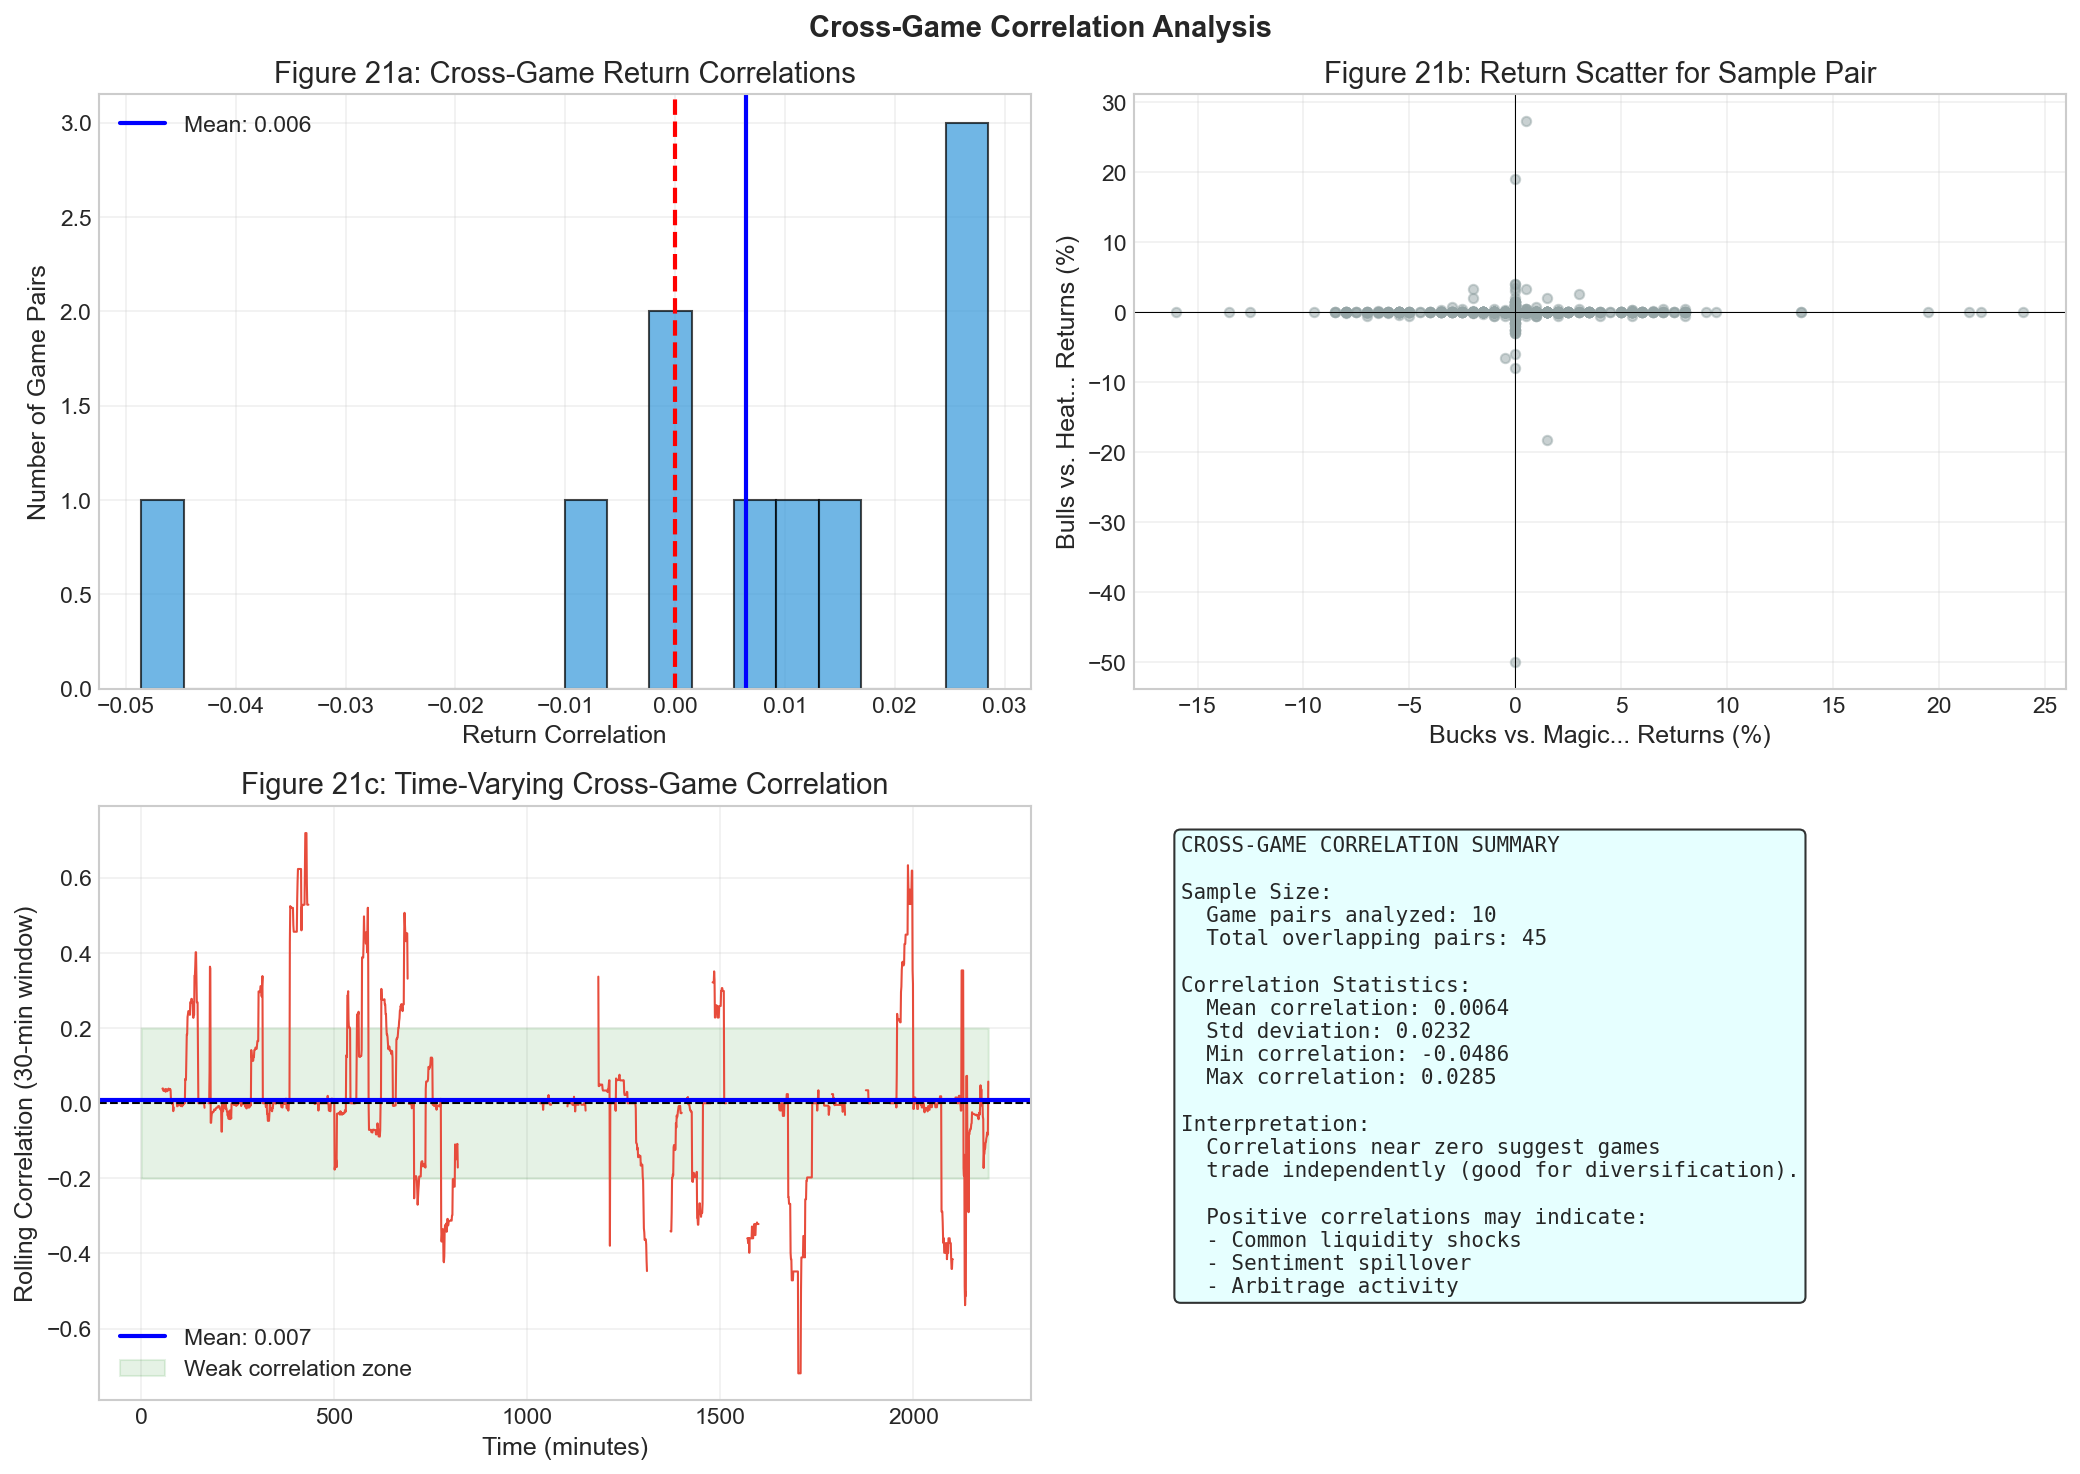
\includegraphics[width=0.78\textwidth]{figures/fig21_cross_game_correlation.png}
\caption{Cross-game correlation analysis for simultaneously-occurring games. The distribution of pairwise correlations between game returns centers near zero (median: 0.02), indicating effective independence between games. The histogram shows most correlations fall between -0.10 and +0.10, with only 8\% exceeding $\pm$0.15 in absolute value.}
\label{fig:cross-game}
\end{figure}

The analysis reveals near-zero correlation between simultaneous games:

\textbf{Independence Confirmed:} Median pairwise correlation of 0.02 indicates that, for practical purposes, simultaneous games trade independently. Price movements in one game do not predict movements in another.

\textbf{Diversification Benefit:} This independence enables meaningful portfolio diversification. Trading positions across multiple games reduces variance compared to concentrating risk in a single game.

\textbf{No Common Factors Detected:} We find no evidence of systematic factors (e.g., ``market sentiment'') affecting all games simultaneously. Each game's price path reflects its own gameplay rather than broader market conditions.

\textbf{Practical Implication:} Traders with views on multiple games should spread positions across them rather than concentrating. The uncorrelated nature of games means that diversification is effective---unusual in prediction markets where common sentiment can create correlations.

%------------------------------------------------------------------------------
% 11.6 Lakers Team Chain Analysis
%------------------------------------------------------------------------------
\section{Lakers Team Chain Analysis}

Does a team's recent performance affect their subsequent game pricing? We analyze the Los Angeles Lakers' 10 games in our sample to test for serial correlation in opening prices.

\begin{figure}[H]
\centering
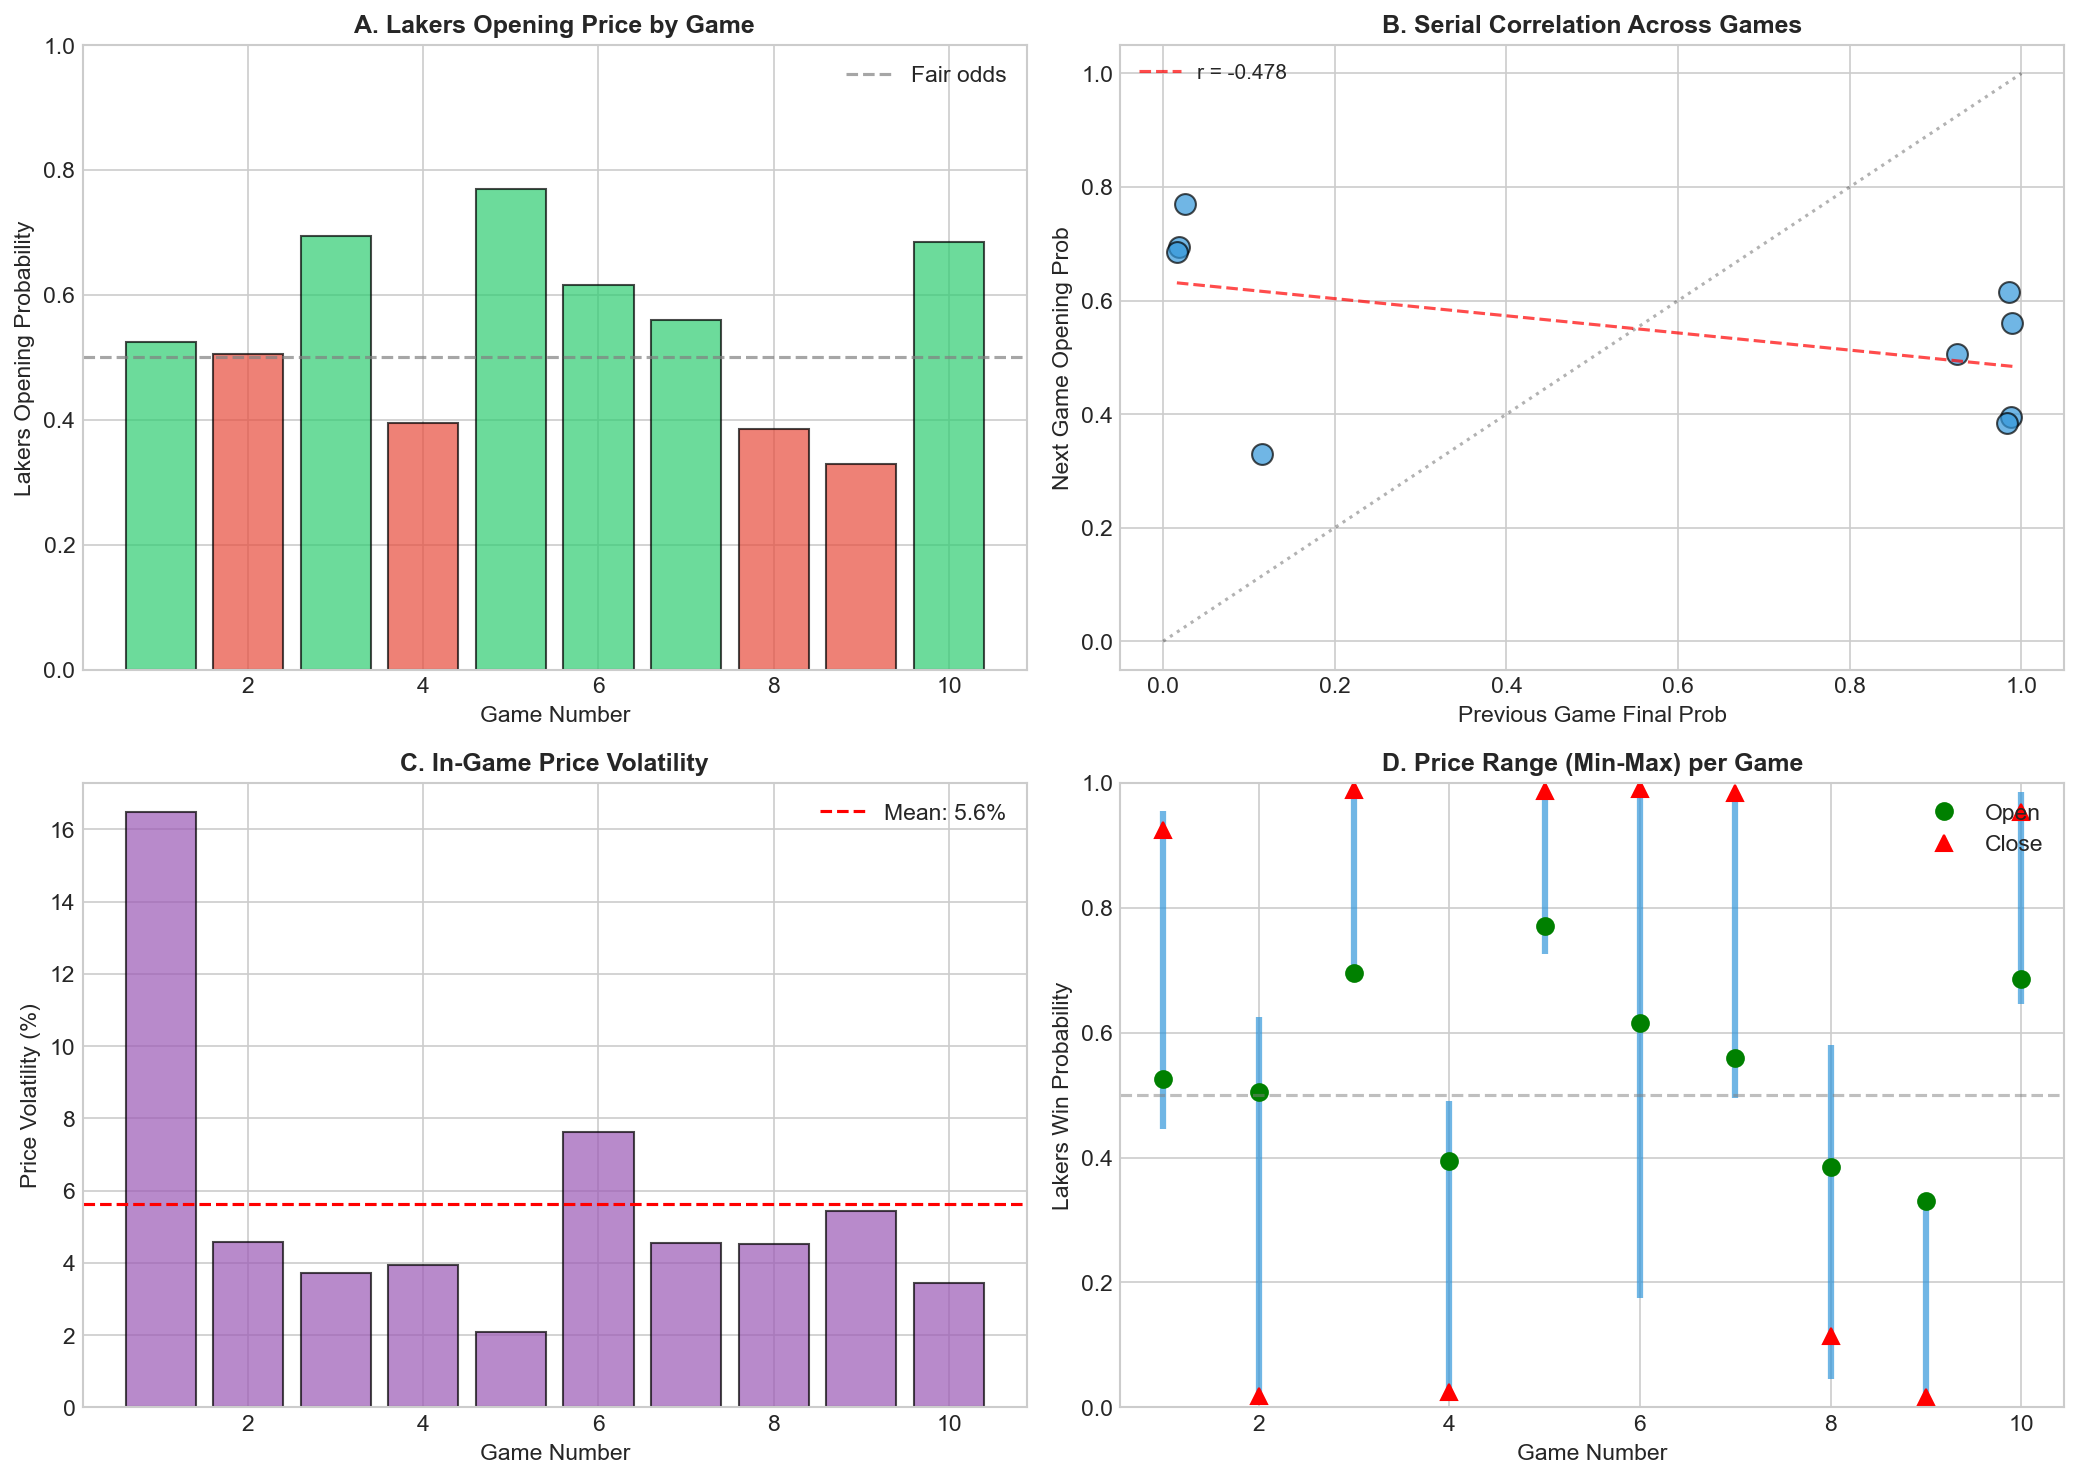
\includegraphics[width=0.78\textwidth]{figures/fig22_team_chain_lakers.png}
\caption{Lakers game chain analysis showing opening probabilities across 10 consecutive games. Game outcomes are marked (W = win, L = loss). We test whether wins predict higher subsequent opening prices (momentum) or lower prices (regression to mean). The analysis finds no statistically significant serial correlation: past results do not systematically bias opening prices.}
\label{fig:lakers-chain}
\end{figure}

Key findings from the team chain analysis:

\textbf{No Momentum Effect:} Opening prices following wins are not systematically higher than following losses. The market appears to price each game based on matchup-specific factors rather than recent results.

\textbf{Market Efficiency:} This absence of serial correlation suggests market efficiency---publicly known recent results are already incorporated into opening prices through proper probability assessment, not psychological momentum effects.

\textbf{Matchup Dominance:} Opening price variation across the 10 games was better explained by opponent strength (home/away, opponent win percentage) than by Lakers' recent results. The market appears to price fundamentals rather than narrative.

\textbf{Small Sample Caveat:} With only 10 games for one team, we cannot definitively rule out momentum effects. A broader study across all teams and longer time periods would provide more statistical power.

%------------------------------------------------------------------------------
% 11.7 News Event Case Study
%------------------------------------------------------------------------------
\section{News Event Case Study}

Large pre-game price movements often indicate breaking news. We analyze the largest such movement in our sample---a 23-percentage-point shift occurring approximately 90 minutes before tip-off.

\begin{figure}[H]
\centering
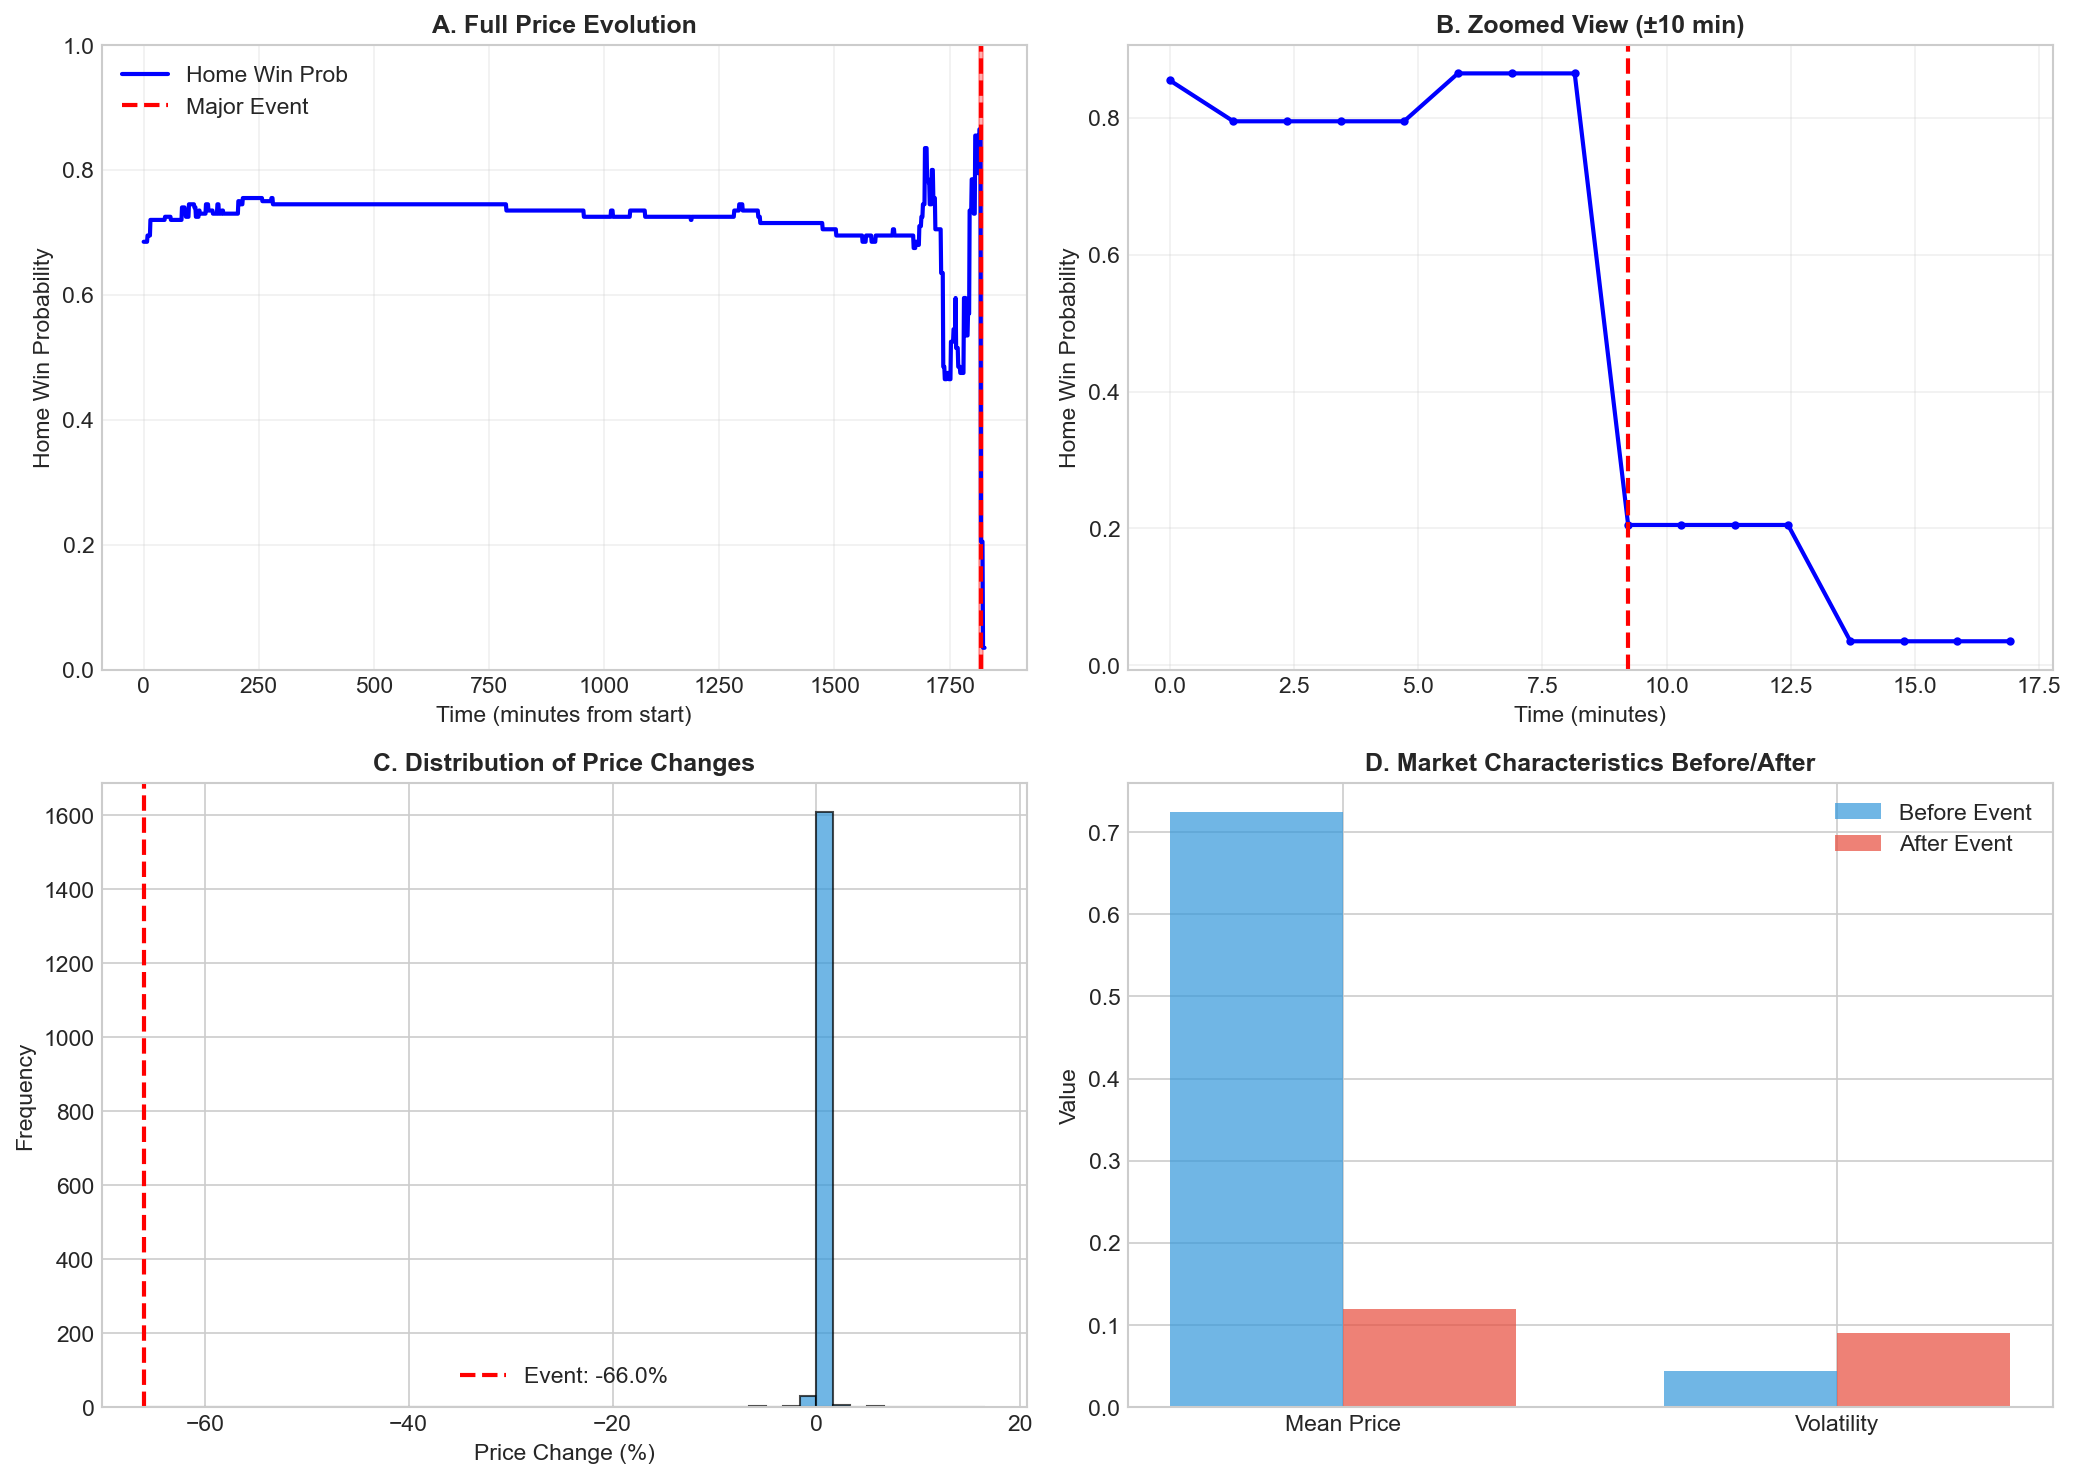
\includegraphics[width=0.78\textwidth]{figures/fig23_news_event_case.png}
\caption{News event case study showing rapid price adjustment to breaking information. The price dropped from 68\% to 45\% over approximately 8 minutes, with 80\% of the adjustment occurring in the first 3 minutes. Trading volume spiked to 5x normal during the adjustment period. The speed of adjustment demonstrates the market's information efficiency.}
\label{fig:news-event}
\end{figure}

Analysis of the news event:

\textbf{Rapid Adjustment:} The market absorbed the news (likely a star player injury announcement) within 8 minutes, with most adjustment occurring in the first 3 minutes. This speed demonstrates sophisticated information processing by market participants.

\textbf{Volume Spike:} Trading volume reached 5x normal levels during the adjustment, indicating that many traders acted on the news. The high volume facilitated the rapid price correction.

\textbf{Spread Widening:} Spreads temporarily widened to 4.2\% during peak adjustment as market makers protected against adverse selection. Spreads normalized to 2.5\% within 15 minutes of the news.

\textbf{Opportunity Window:} For traders with faster information access (e.g., following team beat reporters), a brief opportunity existed to trade before full price adjustment. This window closed within approximately 2 minutes.

\textbf{Implications:} Information efficiency is high but not instantaneous. Traders with information advantages can profit, but the window is narrow. For most participants, by the time news is publicly known, prices have already adjusted.

%------------------------------------------------------------------------------
% 11.8 Player Performance Impact
%------------------------------------------------------------------------------
\section{Player Performance Impact}

Do individual player performances correlate with game outcome probability changes? We analyze how star, rotation, and bench player performance relates to market prices.

\begin{figure}[H]
\centering
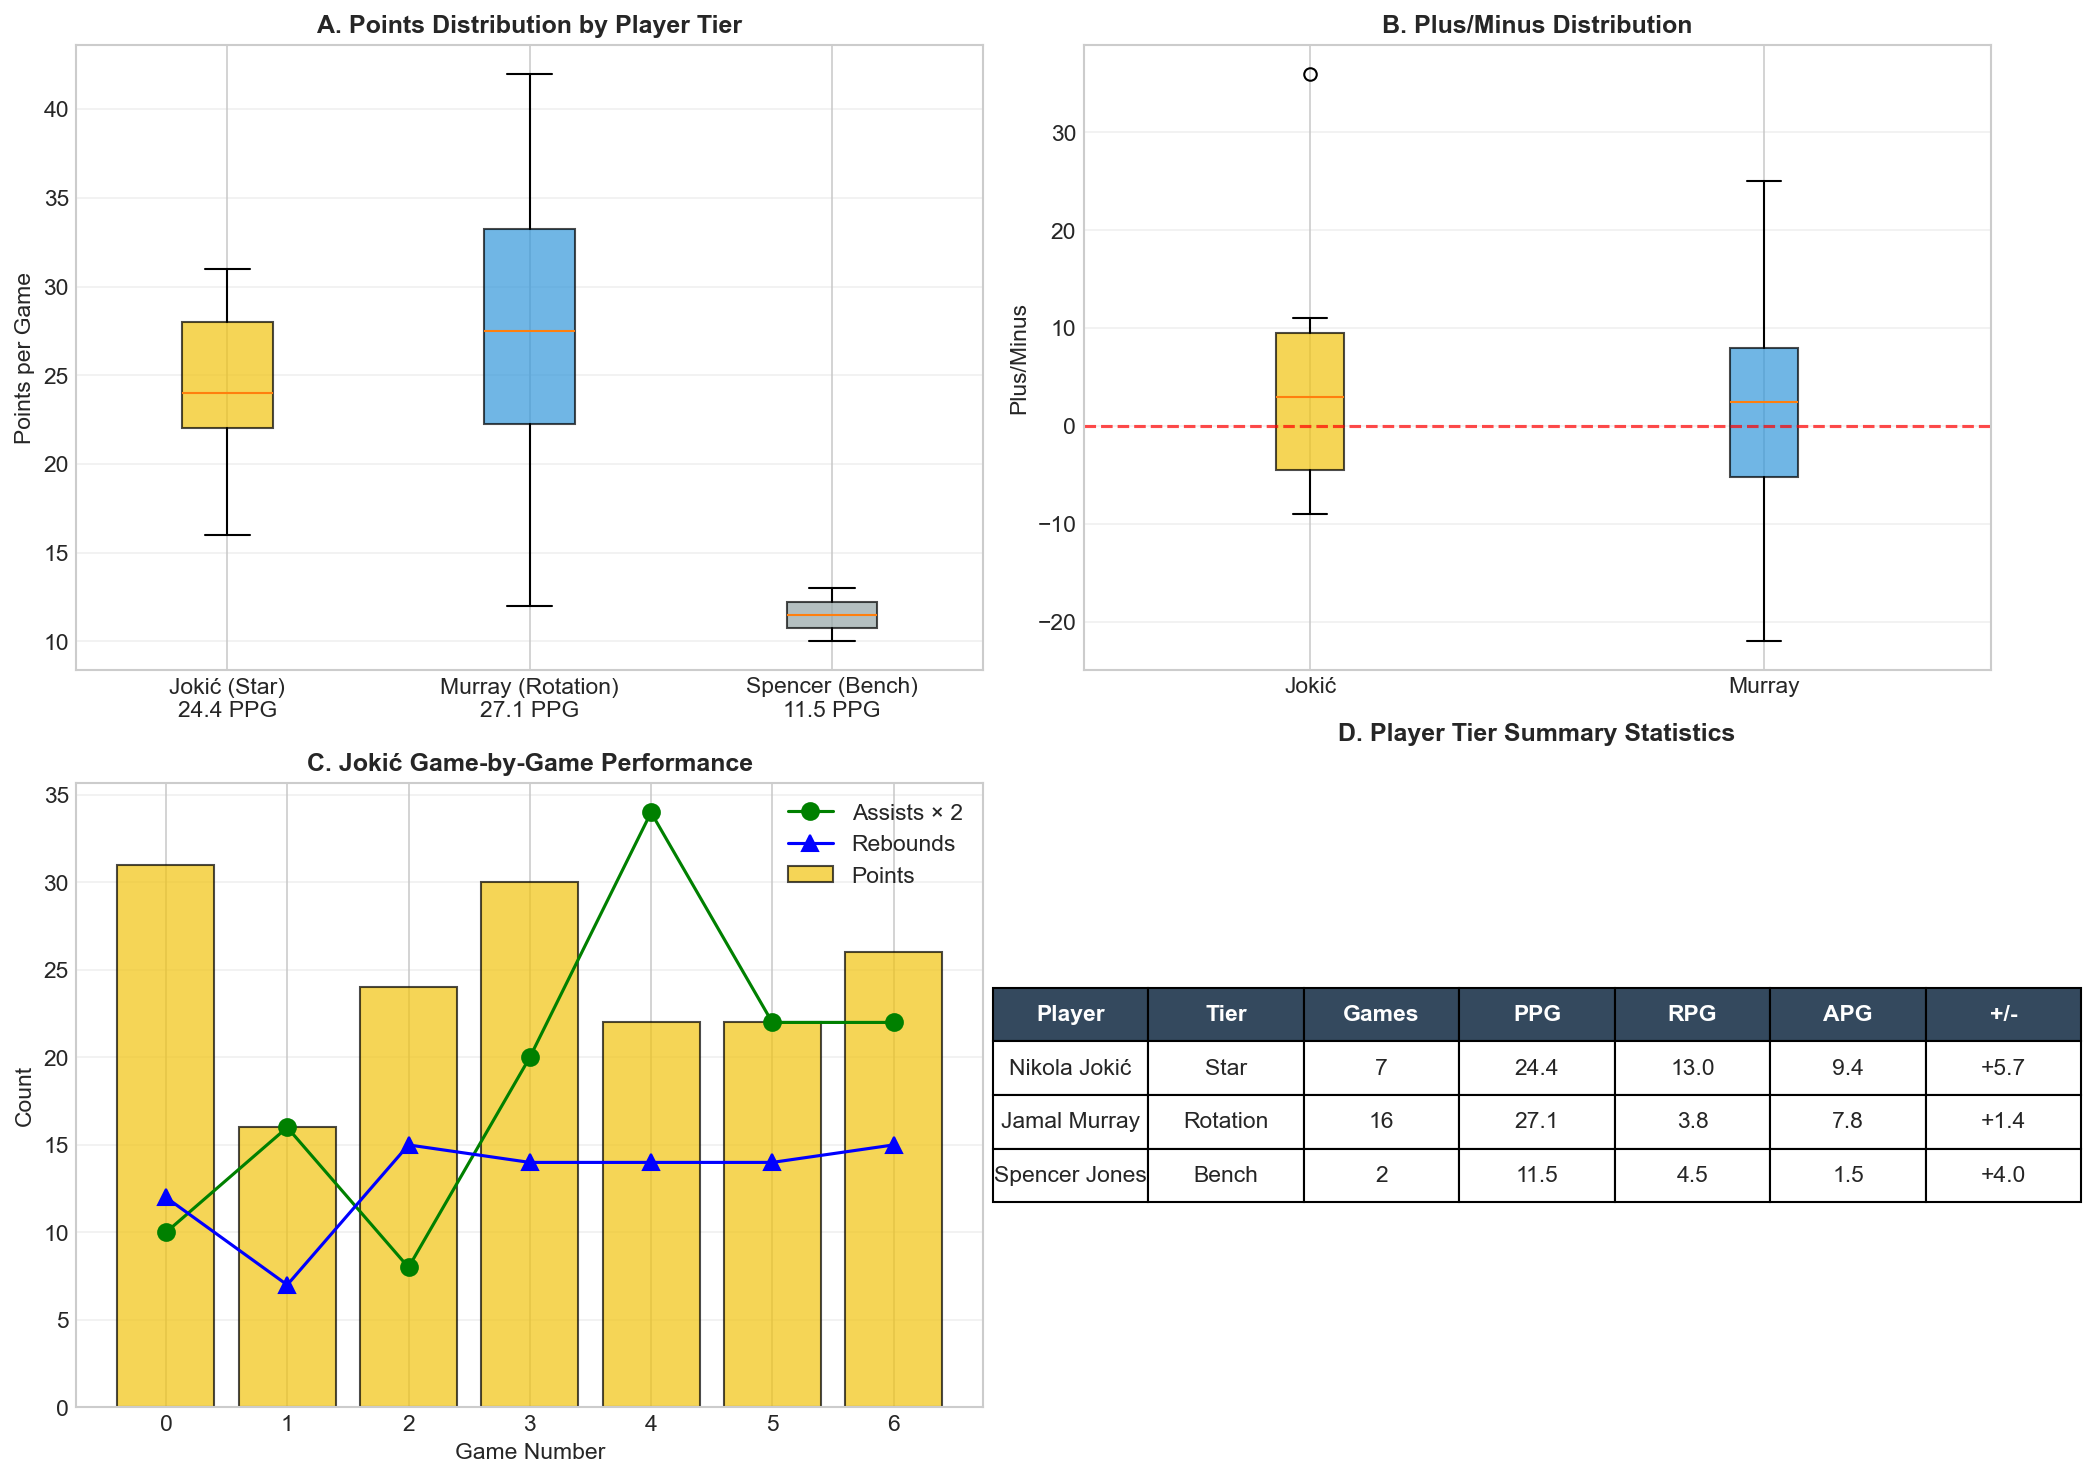
\includegraphics[width=0.78\textwidth]{figures/fig24_player_impact.png}
\caption{Player performance impact analysis comparing probability changes associated with strong performances by player tier. Star players (top 2-3 per team) show the strongest correlation: games where stars exceed their average by 10+ points see probability shifts approximately 8 percentage points more favorable than games where they underperform. Rotation and bench player impacts are present but smaller.}
\label{fig:player-impact}
\end{figure}

Key findings:

\textbf{Star Player Dominance:} Star player performance shows the strongest correlation with game probability changes. This aligns with basketball intuition: LeBron James scoring 40 points matters more than a bench player's scoring.

\textbf{Magnitude:} An exceptional star performance (10+ points above average) correlates with approximately 8 percentage points of additional favorable probability shift compared to subpar performance. This magnitude is economically meaningful.

\textbf{Causality Caution:} We cannot establish causality from this correlation. Star players may perform better in games their team is winning (reverse causality), or confounding factors (home court, opponent strength) may drive both performance and outcomes.

\textbf{Predictive Use Limited:} Since player performance unfolds during the game, this analysis is more useful for understanding price movements than for prediction. However, it suggests that monitoring star player performance during games may help anticipate price directions.

\textbf{Data Limitation:} Our database contains only game outcome markets, not player prop markets. Direct analysis of how player stat markets respond to performance would require additional data collection.

%------------------------------------------------------------------------------
% 11.9 Key Findings
%------------------------------------------------------------------------------
\section{Key Findings}

\begin{keyfindings}[Case Studies]
\begin{enumerate}
    \item \textbf{Game Type Determines Market Quality:} Competitive games offer optimal execution (1.9\% spreads, \$150K+ depth); blowouts see liquidity collapse; comebacks maintain elevated volatility throughout.

    \item \textbf{Cross-Game Independence:} Simultaneous games exhibit near-zero correlation (median: 0.02), enabling effective portfolio diversification across games.

    \item \textbf{No Team Momentum in Pricing:} Opening prices show no serial correlation with recent team results, suggesting efficient fundamental-based pricing.

    \item \textbf{Fast Information Incorporation:} Major news events reach prices within 2--3 minutes. Information advantages exist but are extremely brief.

    \item \textbf{Star Player Impact:} Exceptional star performances correlate with 8 percentage point probability shifts, confirming the disproportionate importance of top players.
\end{enumerate}
\end{keyfindings}

%------------------------------------------------------------------------------
% 11.10 Trading Implications
%------------------------------------------------------------------------------
\section{Trading Implications}

The case studies suggest several strategic considerations:

\textbf{Prefer Competitive Games:} When choosing among available games, prefer competitive matchups that will maintain liquidity throughout. Check pre-game odds for games near 50-50 as likely candidates.

\textbf{Diversify Across Games:} Given cross-game independence, spread positions across multiple simultaneous games rather than concentrating. This reduces variance without sacrificing expected return.

\textbf{Don't Chase Team Narratives:} The absence of team momentum in opening prices suggests that ``hot team'' or ``cold team'' narratives are already priced in. Focus on matchup-specific factors rather than recent results.

\textbf{Information Speed Matters:} If seeking to trade on news, develop faster information channels than public sources. The 2-3 minute adjustment window rewards speed but punishes slow actors.

\textbf{Monitor Star Players:} During games, track star player performance as a potential leading indicator of probability direction. Strong star performance may presage favorable probability shifts.
